\documentclass[a4paper]{article}
%\\\\\\\\\\\\\\\\\\\\\\\\\\\
%Packages en uso

%Idiomas diccionario
\usepackage[english, spanish]{babel}
%\usepackage[english]{babel}

\usepackage[utf8x]{inputenc}
%\usepackage[latin1]{inputenc} 
%\usepackage[ansinew]{inputenc}
\usepackage{ucs}



\usepackage[margin=2cm,portrait,a4paper]{geometry}
%\usepackage[margin=1cm, paperwidth=21.0cm, paperheight=29.6cm]{geometry}

%\usepackage[strict]{changepage}



\usepackage[T1]{fontenc} 
\usepackage{graphicx}
\usepackage{float}
\usepackage{longtable}
%\usepackage{floatflt}
\usepackage{fancyhdr}
\usepackage{hyperref}
%\usepackage{url}
\usepackage{amsfonts}
\usepackage{amssymb}
\usepackage{textcomp}
%\usepackage[symbol]{footmisc}
%\usepackage{pst-circ}
%\usepackage{epsfig}
%\usepackage{xkeyval}
\usepackage{tabularx}
\usepackage{booktabs}


%\usepackage{color}
\usepackage[usenames,dvipsnames]{color}


%\usepackage{minted}
\usepackage{latexsym}
\usepackage{colortbl}
%\usepackage{pdfpages}
\usepackage{wrapfig}

%\usepackage{listings}
\usepackage{listingsutf8}
%\usepackage{mips}
\usepackage{appendix}
\usepackage{needspace}
\usepackage{ifplatform}
\usepackage{ifthen}



%\\\\\\\\\\\\\\\\\\\\\\\\\\\
% FOR GNUPLOT
%\usepackage{tikz}

%\usepackage[miktex]{gnuplottex}
%\usepackage{gnuplot-lua-tikz}
%\usepackage{mathpazo}
%\\\\\\\\\\\\\\\\\\\\\\\\\\\


%\\\\\\\\\\\\\\\\\\\\\\\\\\\
% FOR FIGURE CAPTION COLORS

\usepackage{caption}
\usepackage[svgnames]{xcolor}

%\\\\\\\\\\\\\\\\\\\\\\\\\\\

%\\\\\\\\\\\\\\\\\\\\\\\\\\\
% FOR FIGURE WRAPPING

\usepackage{wrapfig}

%\\\\\\\\\\\\\\\\\\\\\\\\\\\


%\\\\\\\\\\\\\\\\\\\\\\\\\\\
% FOR EQUATION CAPTION FORMAT, COLORS AND OTHERS

\usepackage{amsmath}
\usepackage{mathtools}
\usepackage{bm}

%\\\\\\\\\\\\\\\\\\\\\\\\\\\


%\\\\\\\\\\\\\\\\\\\\\\\\\\\
% TABLES

\usepackage{makecell, multirow, tabularx}
    \newcolumntype{L}{>{\raggedright\arraybackslash}X}
    \renewcommand\theadfont{\normalsize\bfseries\color{white}}
\usepackage{hhline}
\usepackage{setspace}

%\\\\\\\\\\\\\\\\\\\\\\\\\\\


%\\\\\\\\\\\\\\\\\\\\\\\\\\\
% UNITS

\usepackage{siunitx}

\sisetup{output-exponent-marker=\ensuremath{\mathrm{e}}}

%\\\\\\\\\\\\\\\\\\\\\\\\\\\


%\\\\\\\\\\\\\\\\\\\\\\\\\\\
% MATH

\usepackage{mathrsfs}

\usepackage{mathtools}

\usepackage{amsmath,mleftright}

\usepackage{xparse}

\numberwithin{equation}{subsection}

\NewDocumentCommand{\evalat}{sO{\big}mm}{%
  \IfBooleanTF{#1}
   {\mleft. #3 \mright|_{#4}}
   {#3#2|_{#4}}%
}

%\\\\\\\\\\\\\\\\\\\\\\\\\\\

\usepackage{media9}



%\usepackage{showframe}   %% for demo



\begin{document}



%\includemovie[
%	poster,
%	toolbar, %same as `controls'
%	label=kicadampli.u3d,
%	text=(kicadampli.u3d),
%	3Daac=60.000000, 3Droll=0.000000, 3Dc2c=-112.199997 -256.260010 84.849998, 3Droo=292.331238, 3Dcoo=-112.213020 13.163765 -84.848495,
%	3Dlights=CAD,
%]{0.9\paperwidth}{0.9\paperheight}{kicad_ampli.u3d}




%\begin{figure}[H]
%\centering
%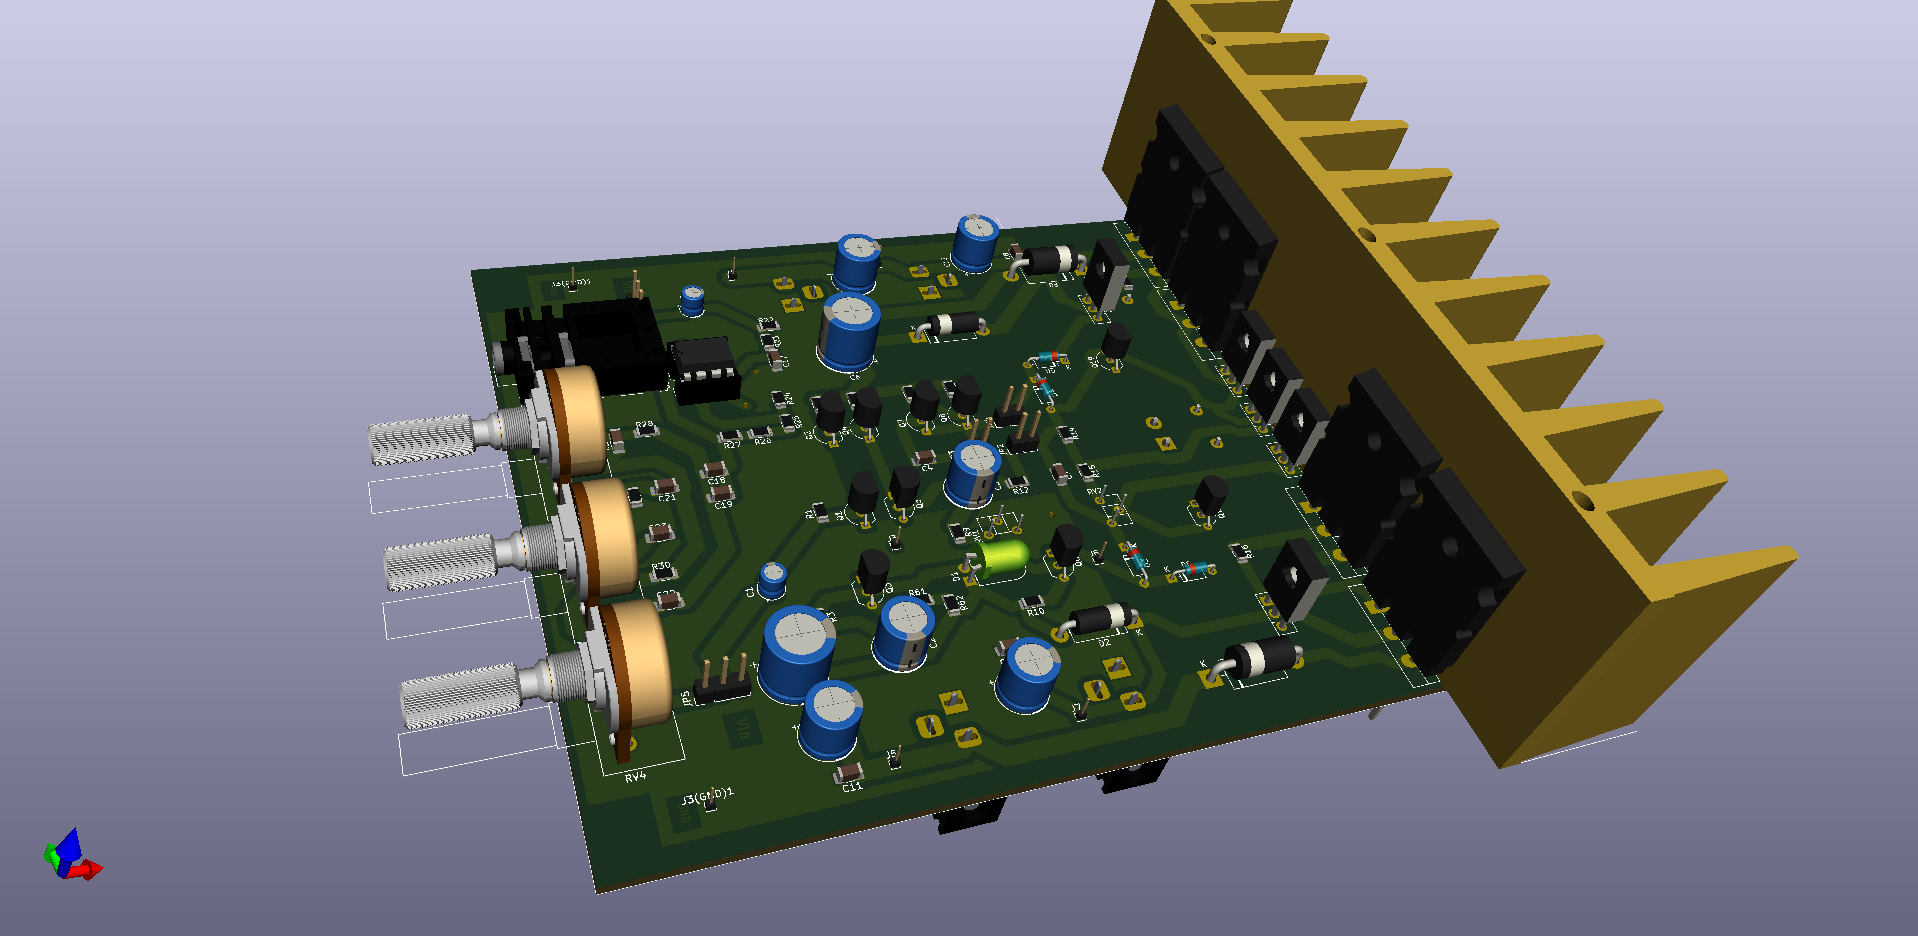
\includegraphics[scale=0.2]{kicad_ampli1.png}
%\end{figure}
%
%
%\clearpage


\section{PCB 3D interactive}


\vspace{3cm}


%\begin{adjustwidth*}{-1.5cm}{-1.5cm}

%\begin{minipage}{0.9\paperwidth}

\begin{figure}[H]
\centering

\includemedia[
width=1.0\linewidth,height=1.0\linewidth,
activate=pageopen,
3Dmenu,
3Droll=64.26156159849816,
3Dc2c=0.8623999357223511 0.44156885147094727 -0.24755491316318512,
3Dcoo=-112.2131118774414 13.16378116607666 -84.84844207763672,
3Droo=469.6991999808034,
3Dlights=Headlamp
]{}{kicad_ampli.u3d}

\end{figure}

%\end{adjustwidth*}




\end{document}
